% This part is the latex header. It defines what kind of document this will be and 
% says which packages to use. Packages let you include different kind of formats
% and templates in the document. 
\documentclass[11pt]{article} % document type - other options are journal or book?
\usepackage[pdftex]{graphicx} % package to import figures
\usepackage{float} % used for placing figures - H
\usepackage{hyperref} % used for including links (hyper links)
\usepackage{enumerate} % used for making lists
\usepackage[margin=1cm]{geometry}
\usepackage{tabularx}
\usepackage{booktabs}
\usepackage{amsmath}
\usepackage[version=3]{mhchem} 
\usepackage{siunitx}

% math packages
\usepackage{amssymb}
\usepackage{amsmath}

\pagestyle{headings}
\topmargin -0.5in
\oddsidemargin 0.0in
\textwidth 6.5in
\textheight 9.0in

% declare the title, date and author
\title{Radial Bias Pilot 1}
\date{Jan 20, 2021}
\author{Rania Ezzo}

% This is where the actual document starts
\begin{document}
\maketitle
\tableofcontents


\section{Goal of Pilot 1}
To measure radial direction bias with 1D drifting gratings at 2-4 polar angle locations at a given eccentricity. A total of 4 directions of motion will be tested, 2 radial (inwards and outwards) and 2 tangential (clockwise, counterclockwise), to measure the performance differences between (1) centrifugal and centripetal motion directions, and (2) radial and tangential motion directions. 

\subsection{Parameters}
Eccentricity from central fixation: 7 degrees
\\
Locations tested (polar angle relative to fixation): Upper left (45 deg) and lower right (225 deg)
\\
Stimulus: sine wave gratings w/ gaussian mask
\\
Stimulus spatial frequency: 1 c/deg
\\
Stimulus drift speed: 4 deg/s
\\
Stimulus contrast: full contrast + gaussian mask
\\
Stimulus aperature diameter: 2.5 deg
\\
Black circular aperature was put onto screen to avoid perceptual artifacts from screen edges
\\
Number of subjects: 1

\subsection{Experimental Design}
The pilot uses a 2AFC paradigm, where each trial includes a drifting grating presented at 1 of 2 possible positions, while the subject maintains fixation at the central dot. A method of constant stimuli is used which is set based on the performance of the training session (see Methods). The angular values added to the internal reference frame is chosen at random from the following constants [-8, 6, 5, 3, 2.5, 2, 1, 0, 1, 2, 2.5, 3, 5, 6, 8]. The observer must determine whether the direction of motion if clockwise or counterclockwise relative to the internal reference. The sequence of each trial is depicted below:

\begin{figure}[H]
\centering % centers the figure
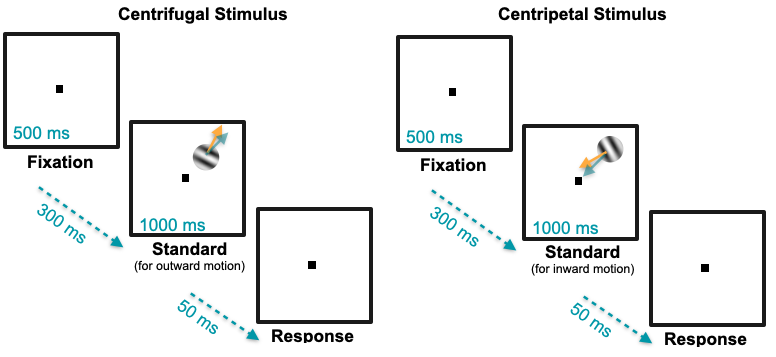
\includegraphics[scale=.4]{Images/Radial_sequence.png}
\\
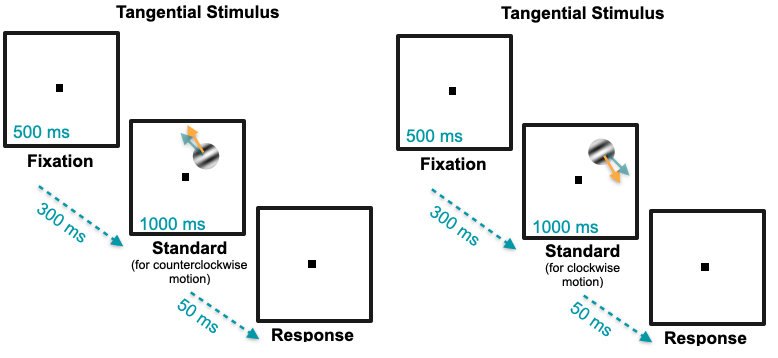
\includegraphics[scale=.4]{Images/Tang_sequence.png}
\end{figure}

\subsection{Block sequence}
Four blocks were run, and each block corresponded to 1 of the 4 conditions being tested (tangential counterclockwise motion, tangential clockwise motion, radial outwards motion, radial inwards motion). The internal reference frames for each block is shown below:

\begin{figure}[H]
\centering % centers the figure
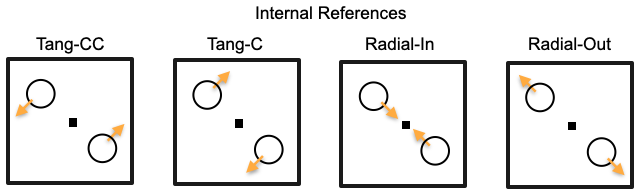
\includegraphics[scale=.4]{Images/Blocks.png}
\end{figure}

Prior to the experiment, the 2 "standard" motion directions corresponding to that block are showed to observer to use as an internal reference. Then a training session is conducted to determine how much tilt is required to meet 75\% accuracy with staircase procedure (MLPest), and to allow subject to practice task with feedback. This was tested using radial motion only, and ~2.5 degrees was the estimated angular value to add/subtract to the standard to achieve 75\% performance of the clockwise/counterclockwise discrimination task. Constants [-8, -6, -5, -3, -2.5, -2, -1, 0, 1, 2, 2.5, 3, 5, 6, 8] were chosen to roughly center around this value for all 4 conditions. Note positive and negative values for clockwise v. counterclockwise tilt.
\\
Each block contains (2 locations with clockwise/counterclockwise motion) x 80 repetitions = 1,280 trials. All 4 full-blocks took 80 min. 
\\
Sequence of half-blocks tested: 
\begin{enumerate}
\item radial-out [angles: +- 8, 6, 5, 3]
\item radial-in [angles: +- 8, 6, 5, 3]
\item tang-cc [angles: +- 8, 6, 5, 3]
\item tang-c [angles: +- 8, 6, 5, 3]
\item tang-c [angles: +- 2.5, 2, 1, 0]
\item tang-cc [angles: +- 2.5, 2, 1, 0]
\item radial-in [angles: +- 2.5, 2, 1, 0]
\item radial-out [angles: +- 2.5, 2, 1, 0]
\end{enumerate}

\section{Data}
\subsection{Psychometric Function (Cumulative normal)}
\begin{figure}[H]
\centering % centers the figure
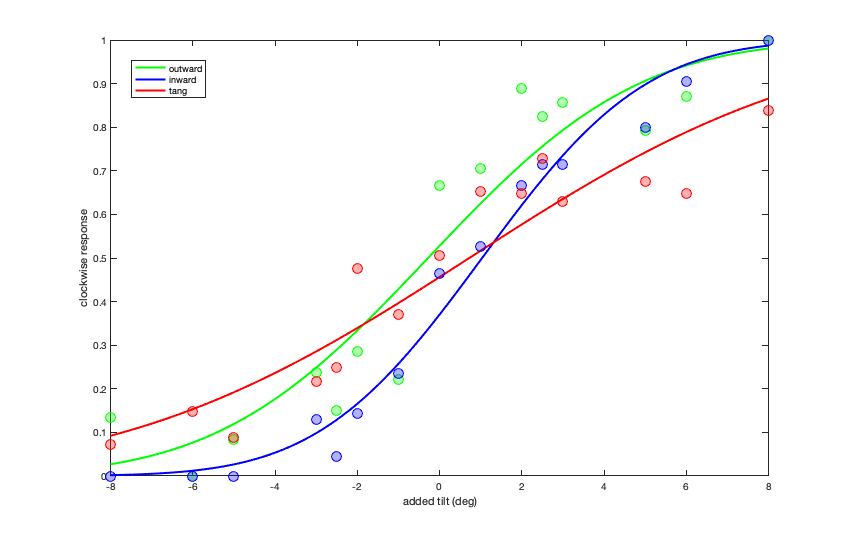
\includegraphics[scale=.4]{Images/PF_angles.png}
\end{figure}

\newpage
\subsection{Current number of trials}
N\_Trials is the total number of trials for a particular condition.
Ans\_clock is the percentage of the observer answering clockwise out of the N\_Trials for that condition.
\begin{table*}[htb]
  \label{tbl:stats-and-correlations}
  %\small\begin{tabularx}{\linewidth}{X*{15}{c}}
  \small\begin{tabular*}{\linewidth}{l@{\extracolsep{\fill}}*{15}{c}}
    \toprule
    & \multicolumn{4}{c}{\textbf{Radial outwards}}\\ \cmidrule(r){2-13}
    & {-8} & {-6} & {-5} & {-3} & {-2.5} & {-2} & {-1} & {0} & {1} & {2} & {2.5} & {3} & {5} & {6} & {8} \\ [0.5ex]
    N\_Trials &    15 &    20 &    24 &    21 &    20 &    21 &    18 &    48 &    17 &    18&    17&    14&    24&    23&    19\\
    Ans\_clock &    .13 &    .0 &    .08 &    .24 &    .15 &    .29 &   .22 &    .67&    .71&    .89&    .82&    .86&    .79&    .87&    1.0\\
    \bottomrule
  %\end{tabularx}
  \end{tabular*}
\end{table*}

\begin{table*}[htb]
  \label{tbl:stats-and-correlations}
  %\small\begin{tabularx}{\linewidth}{X*{15}{c}}
  \small\begin{tabular*}{\linewidth}{l@{\extracolsep{\fill}}*{15}{c}}
    \toprule
    & \multicolumn{4}{c}{\textbf{Radial inwards}}\\ \cmidrule(r){2-13}
    & {-8} & {-6} & {-5} & {-3} & {-2.5} & {-2} & {-1} & {0} & {1} & {2} & {2.5} & {3} & {5} & {6} & {8} \\ [0.5ex]
    N\_Trials &    22 &    18 &    17 &    23 &    22 &    14 &    17 &    41 &    19 &    18&    28&    28&    15&    21&    16\\
    Ans\_clock &    .0 &    .0 &    .0 &    .13 &    .05 &    .14 &   .24 &    .46&    .53&    .67&    .71&    .71&    .8&    .9&    1.0\\
    \bottomrule
  %\end{tabularx}
  \end{tabular*}
\end{table*}

\begin{table*}[htb]
  \label{tbl:stats-and-correlations}
  %\small\begin{tabularx}{\linewidth}{X*{15}{c}}
  \small\begin{tabular*}{\linewidth}{l@{\extracolsep{\fill}}*{15}{c}}
    \toprule
    & \multicolumn{4}{c}{\textbf{Tangential (combined)}}\\ \cmidrule(r){2-13}
    & {-8} & {-6} & {-5} & {-3} & {-2.5} & {-2} & {-1} & {0} & {1} & {2} & {2.5} & {3} & {5} & {6} & {8} \\ [0.5ex]
    N\_Trials &    41 &    34 &    34 &    51 &    48 &    42 &    35 &    77 &    46 &    37&    33&    46&    40&    37&    37\\
    Ans\_clock &    .07 &    .15 &    .09 &    .22 &    .25 &    .48 &   .37 &    .51&    .65&    .65&    .73&    .63&    .68&    .65&    .84\\
    \bottomrule
  %\end{tabularx}
  \end{tabular*}
\end{table*}

\section{Feedback from Jon and Bas} 
\begin{itemize}
\item Calculate bias (alpha), and slope for the PFs
\item Change blocks to include vectors of the same direction so the subject does not have to change internal reference frame within block
	\begin{itemize}
	\item For example, include radial for upper left and radial inward for lower right in one block, etc.
	\end{itemize}
\item Run experiment 2x (once for each block) to a test-retest validation, and plot.
\item Make sure to run an equal number of trials (sample without replacement).
\item Leave out condition with 0 degrees added tilt (not needed).
\item Include feedback for all trials to reinforce knowledge of internal stimulus.
\end{itemize}

\end{document}